\section{Scope and definitions}
\label{sec:scope}

\subsection{Scope}

This document is the official project management protocol for the Netherlands eScience Center. It describes all phases
of a project and the procedures required to successfully complete them.

The scope of this document is the execution of research projects awarded by the eScience Center through calls for
proposals, though other types of projects are also briefly covered. This document gives a detailed description of all
steps, both necessary and optional, that must or may be taken in the execution of projects, reflecting the so-called
\textit{project life cycle}. For each step, the document indicates the responsibilities of the project team members
(RSEs) and other eScience Center employees (e.g. Programme Managers, Finance, Directors Team) involved in the
process.

Call procedures follow a separate protocol~\cite{call-protocol-2015} and are
not covered by this document. The call procedure protocol ends with the formal awarding of projects by the eScience
Center Governing Board or the Directors Team (DT), the notification of Lead Applicants and the formalization of the
awarding by means of a \textit{toekenningsbrief} ('Awarding letter’). The
current document describes all activities that (need to) take place from that moment onwards, until the formal closing
of the project. An independent evaluation of projects, including impact, output, process and collaboration with project
partners is outside of the scope of the current document, and will be published as a separate document or a subsequent
version of this document in the future. 

This document has been approved by the DT and will be subject to evaluation and possible adaptation annually.

The structure of this document largely follows the project life cycle (see Section~\ref{sec:scope:lifecycle}); the
protocol describes activities in chronological order.

\subsection{Stakeholders}
An eScience project is a project involving the eScience Center, where responsibility is shared between different
stakeholders who each have their own roles and responsibilities during specific phases of the project.


%\resizebox{\textwidth}{!}{%
%\begin{tabular}{p{0.15\textwidth}p{0.15\textwidth}p{0.2\textwidth}p{0.2\textwidth}p{0.1\textwidth}}
\begin{tabularx}{\linewidth}{p{0.12\textwidth}|p{0.12\textwidth}|p{0.12\textwidth}|p{0.25\textwidth}|p{0.25\textwidth}}
\toprule
\textbf{Stakeholder} & \textbf{Abbreviation} & \textbf{Assignment}& \textbf{Role}& \textbf{More info}\\
\midrule
\endfirsthead
\toprule
\textbf{Stakeholder} & \textbf{Abbreviation} & \textbf{Assignment}& \textbf{Role}& \textbf{More info}\\
\toprule
\endhead
\midrule
\multicolumn{5}{r}{}
\endfoot
\bottomrule
\endlastfoot  
Lead Applicant & LA & main applicant and recipient of the grant & primary contact for the eScience Center project, accountable for the (quality of the) scientific contribution to the project & responsibilities defined in the call text, Terms and Conditions, and possibly a Consortium/Collaboration agreement.  \\\hline
Programme Manager                                  & PM                    & assigned by the PM team~\footnote{All PMs, led by the Programme Director, constitute the PM team.}                                                                                          & accountable for the eScience contribution, delivering results within scope, time, and budget; project budget holder                                                              & Full text of responsibilities available in the PM job profile document and PM mandate (see~\cite{intranet})  \\\hline
Lead Research Software Engineer                    & Lead RSE              & appointed by accountable PM                                                                                       & responsible for the timely execution of the project, main contact person for the project with other stakeholders                                                                                                                       & More details on responsibilities, see the formal role description of Lead RSE (Appendix~\ref{app:leadRSE}).                          \\\hline
Research Software Engineer (assigned to a project) & RSE                   & assigned by the accountable PM                                                                                    & responsible for the timely completion of the project                                                                                                                                                                                   & Definition given in~\cite{rse}. All RSE activities coordinated by Lead RSE in agreement with PM.                                                                     \\\hline
Consulting Research Software Engineer              & Consulting RSE        & involved at request of Lead RSE or accountable PM                                                                 & provides expertise to the project for a defined period; may also join key meetings in addition to an expertise contribution                                                        & All activities coordinated by Lead RSE in agreement with PM in case the project team needs additional expertise.                     \\\hline
Technology Lead.                                    & TL                    & assigned by the TL team~\footnote{All TLs, led by Director of Technology, constitute the TL team.}                & acts as point of contact for Lead RSE to the TL team. Safeguards the technological aspects of a project; accountable for the quality, reuse and sustainability of the research software developed.                                     & The TLs team is responsible for internal training programme of RSEs.                                                                 \\\hline
Section Head                                       & SH                    & assigned by the PM/SH team~\footnote{All SHs, led by Executive Director, constitute the SH team.}                 & line manager of RSEs, responsible for monitoring the overall effectiveness of RSEs in bringing projects to completion; maintain overview of a research domain.                                                                         & The SH team assigns one SH to each RSE team, and the SH ensures that team keeps its capacity and planning up to date.                \\\hline
Communica-tions                                     &                       &                                                                                                                   & advise and support internal and external project communication, including showcasing through news, website, newsletters, social media, interviews, and videos.                                &                                                                                                                                      \\\hline
Community Manager                                  & CM                    &                                                                                                                   & advise on developing outreach activities and promoting community engagement, responsible for external training programme                                                                                                               &                                                                                                                                      \\\hline
Secretary                                          &                       &                                                                                                                   & organizes formal meetings, provide with agenda and slide template, invitation text, list of participants (with emails), and timeline.                                                                                                  &                                                            \\\hline
Programme Director                                 & PD                    &                                                                                                                   & the escalation point for PMs and liaison to DT for project-related decisions; approves workshop plans (with Finance) and holds the Acquisition budget. &                                                                                                                                      \\\hline
Director of Technology                             & DoT                   &                                                                                                                   & the escalation point for TLs, the contact point of TLs to DT, accountable (and responsible) for licences and Intellectual Property (IP), software sustainability budgets holder                                                        &                                                                                                                                      \\\hline
Director of Operations                             & DoO                   &                                                                                                                   & handles legal questions (e.g., contracts, Collaborative Agreements and guest agreements)                                                                                               &                                                                                                                                      \\\hline
Finance \& Control                                 & Finance               & part of Operations, includes Controller, and led by DoO                                                           & responsible for maintaining finances and project administration                                                                                                                                                                &                                                                   \\\hline
Directors Team                                     & DT                    & comprised of DoT, DoO, General Director and PD                                                                    & approves formal decisions regarding projects (e.g., budget changes)                                                                                                                                                                    &                                                                                                                                      \\\hline
GDPR contact person                                &                       & appointed by the DT, see the Intranet for contact information                                                     & consults on GDPR~\cite{GDPR} or privacy-related issues in the project                                                                                                                                                                             & The eScience Center has not appointed a Data Protection Officer. GDPR aspects must be discussed with the contact person.             \\\hline
eScience Center project team                       & eScience project team & comprises RSEs, PM and TL working on the project                                                                  & responsible for the timely completion of the project                                                                                                                                                                                   &                                                                                                                                      \\\hline
Project team                                       &                       & comprises the eScience project team, LA and their team (including team members indicated in the project proposal) & responsible for the timely completion of the project                                                                                                                                                                                   &                                                                                                                                      \\\hline
Editorial Team                                     &                       &                                                                                                                   & provides support with outreach                                                                                                                                                                                                         & The eScience Center maintains a blog, and has presence in major social networks                                                     
%\end{tabular}%
%}
\end{tabularx}


\subsection{Types of projects}
The eScience Center receives an annual budget from \href{https://www.nwo.nl/}{NWO} and \href{https://www.surf.nl/}{SURF}, the larger part of which is allocated to projects
submitted by researchers working at eligible research performing organizations in the Netherlands in the form of the
in-kind provision of RSEs. Projects may also be \href{https://research-software-directory.org/organisations/netherlands-escience-center?categories=%5B%22External%22%5D&tab=projects}{funded from external sources} (henceforth referred to as \textit{an
external project) }or funded from the annual budget but carried out internally.

By awarding subsidy to a project or by pledging a contribution to an external project, the eScience Center takes on the
obligation to deliver high-quality work in a timely manner.

\subsubsection{Call projects}
The eScience Center publishes a range of calls. Each project is a part of a specific call (regular calls such as
\href{https://doi.org/10.5281/zenodo.6602691}{OEC}, \href{https://doi.org/10.5281/zenodo.10865584}{SS}, \href{10.5281/zenodo.5163292}{SSI}, or \href{https://research-software-directory.org/organisations/netherlands-escience-center?categories=%5B%22Collaborative%20Calls%22%5D&tab=projects}{calls in collaboration with other funders} such as \href{https://zoek.officielebekendmakingen.nl/stcrt-2019-32775.html}{Big Data \& Health}, 
\href{https://www.nwo-i.nl/wp-content/uploads/2017/03/JCER-call-2017_UK.pdf}{JCER}, \href{https://zoek.officielebekendmakingen.nl/stcrt-2019-54263.html}{ESI-FAR}). Projects from the regular calls before 2021 are partly in-cash, while projects awarded later
are fully in-kind (plus a reserved budget for workshops).

Calls can reserve part of the project or the call budget to serve the eScience Center agenda to increase the impact of
software beyond the project itself. Henceforth this will be referred to as the software sustainability budget, formerly
known as generalization budget). The budget is intended for software generalization, reuse and sustainability, and
community building. The DoT is the holder of this budget. Details concerning this budget are included in the Awarding
letter. See Section~\ref{sec:opportunities:ss} for more information.

Project teams (mainly Lead RSE, PM and TL) are expected to consult legal documents such as the specific call text, Awarding letter
(‘Toekenningsbrief’), Terms and Conditions document (‘Bijzondere voorwaarden’, ‘Subsidieregeling’, etc.), Consortium/Collaboration Agreement (CA), and/or
contracts for grant terms and conditions. The LA is responsible for adhering to the conditions of the project, while
the PM, with the help of the Lead RSE, monitors this.

In our call projects, most of the total requested budget is dedicated to project work and project-related activities.
The remaining part (referred to as “general activities”) covers activities that benefit our ability to contribute to
high-quality research, such as the professional development of RSEs through training, work meetings, conferences, etc,
as well as the administrative coordination and project management within the eScience Center. It is up to the PMs and
RSEs in consultation with the SHs to fairly distribute hours for general activities across all the projects they
contribute to (cf. Section~\ref{sec:exec:budget}). The exact percentage set aside for general activities is defined in
the call within which a project has been awarded.

\subsubsection{External projects}
Projects funded externally by e.g. NWO or the EU, or via private-public partnerships, are governed by external funding
conditions specified in a contract or agreement that may supersede our own rules. %The budgets of these projects need to be approved by Finance and the DoO. 
The LA is responsible for adherence to these rules and conditions, while the Lead RSE monitors this. 
Again, the project team (mostly, Lead RSE, PM, TL) must consult the specific call
text and other formal documents (Awarding letter, Terms and Conditions document, Consortium/Collaboration Agreements, contracts for the conditions
and rules). Projects under external funding are covered partially by this protocol. The formalities around the acquisition process follow the workflow described in “External funding” (see Section
\ref{sec:opportunities:external-funding} for more information).

\subsubsection{Other projects}
This document only briefly covers other types of projects such as those funded through Ambition 2~\cite{nlesc-strategy}, namely Dissemination
\& Community (D\&C), Knowledge \& Development (KD) and Fellowship projects in 
Section~\ref{sec:opportunities:fellowship} and Appendix~\ref{app:pm-role}.

\clearpage
\subsection{Project life cycle overview}
\label{sec:scope:lifecycle}

\begin{figure}[!h]
    \centering
    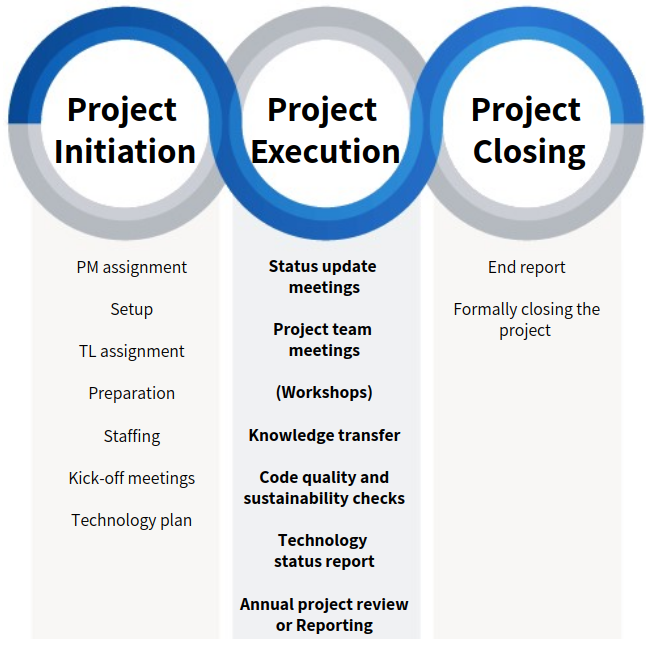
\includegraphics[scale=0.5]{img/lifecycle-stages.png}
    \caption{Project lifecycle stages}
    \label{fig:project-lifecycle}
\end{figure}

At the eScience Center, a standard project life cycle is a three-phase process (see Figure~\ref{fig:project-lifecycle}). First, project stakeholders initiate the
project. Next, the project team executes the project and monitors its progress. Finally, once the project reaches its
end, it is formally closed.

These three phases are covered in detail in the next sections.
